% Created by tikzDevice version 0.12.6 on 2025-04-02 10:49:50
% !TEX encoding = UTF-8 Unicode
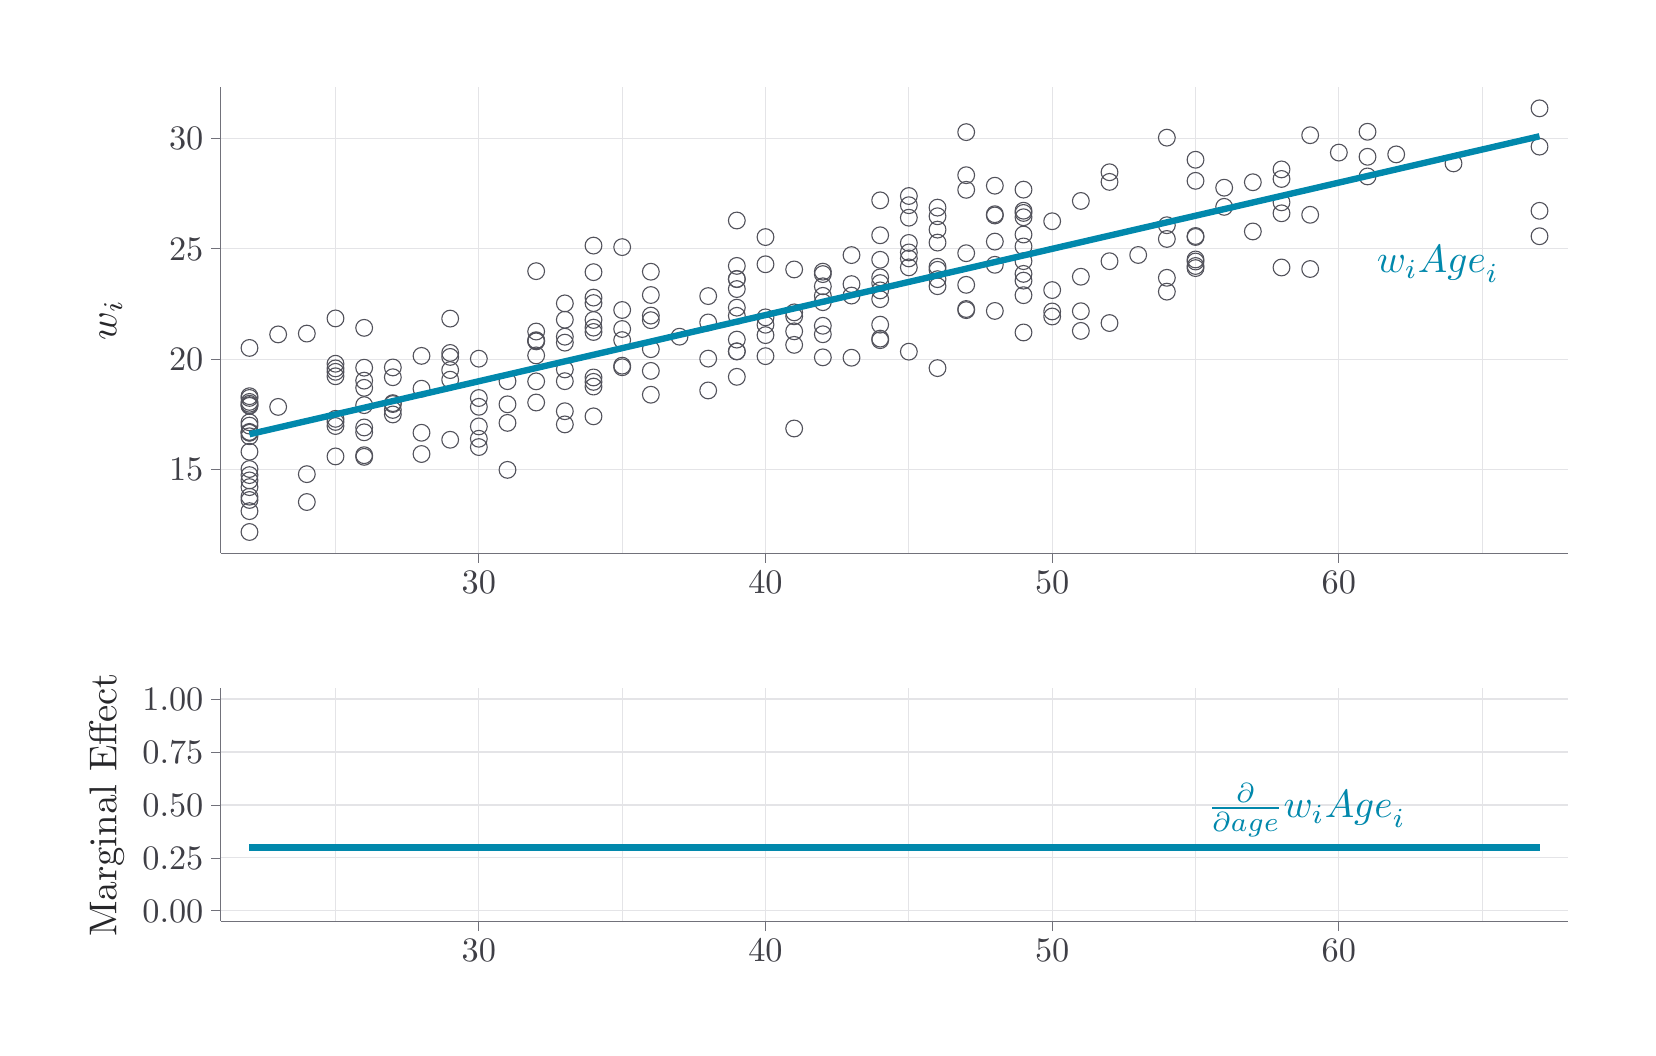
\begin{tikzpicture}[x=1pt,y=1pt]
\definecolor{fillColor}{RGB}{255,255,255}
\path[use as bounding box,fill=fillColor] (0,0) rectangle (578.16,361.35);
\begin{scope}
\path[clip] (  0.00,  0.00) rectangle (578.16,361.35);
\definecolor{drawColor}{RGB}{255,255,255}

\path[draw=drawColor,line width= 0.6pt,line join=round,line cap=round,fill=fillColor] (  0.00,  0.00) rectangle (578.16,361.35);
\end{scope}
\begin{scope}
\path[clip] (  5.50,138.58) rectangle (572.66,355.85);
\definecolor{drawColor}{RGB}{255,255,255}
\definecolor{fillColor}{RGB}{255,255,255}

\path[draw=drawColor,line width= 0.7pt,line join=round,line cap=round,fill=fillColor] (  5.50,138.58) rectangle (572.66,355.85);
\end{scope}
\begin{scope}
\path[clip] (  5.50,  5.50) rectangle (572.66,138.58);
\definecolor{drawColor}{RGB}{255,255,255}
\definecolor{fillColor}{RGB}{255,255,255}

\path[draw=drawColor,line width= 0.7pt,line join=round,line cap=round,fill=fillColor] (  5.50,  5.50) rectangle (572.66,138.58);
\end{scope}
\begin{scope}
\path[clip] ( 69.80,171.46) rectangle (556.66,339.85);
\definecolor{drawColor}{RGB}{255,255,255}
\definecolor{fillColor}{RGB}{255,255,255}

\path[draw=drawColor,line width= 0.7pt,line join=round,line cap=round,fill=fillColor] ( 69.80,171.46) rectangle (556.66,339.85);
\definecolor{drawColor}{RGB}{228,228,231}

\path[draw=drawColor,line width= 0.4pt,line join=round] (111.23,171.46) --
	(111.23,339.85);

\path[draw=drawColor,line width= 0.4pt,line join=round] (214.82,171.46) --
	(214.82,339.85);

\path[draw=drawColor,line width= 0.4pt,line join=round] (318.41,171.46) --
	(318.41,339.85);

\path[draw=drawColor,line width= 0.4pt,line join=round] (422.00,171.46) --
	(422.00,339.85);

\path[draw=drawColor,line width= 0.4pt,line join=round] (525.58,171.46) --
	(525.58,339.85);

\path[draw=drawColor,line width= 0.4pt,line join=round] ( 69.80,201.68) --
	(556.66,201.68);

\path[draw=drawColor,line width= 0.4pt,line join=round] ( 69.80,241.55) --
	(556.66,241.55);

\path[draw=drawColor,line width= 0.4pt,line join=round] ( 69.80,281.43) --
	(556.66,281.43);

\path[draw=drawColor,line width= 0.4pt,line join=round] ( 69.80,321.30) --
	(556.66,321.30);

\path[draw=drawColor,line width= 0.4pt,line join=round] (163.03,171.46) --
	(163.03,339.85);

\path[draw=drawColor,line width= 0.4pt,line join=round] (266.61,171.46) --
	(266.61,339.85);

\path[draw=drawColor,line width= 0.4pt,line join=round] (370.20,171.46) --
	(370.20,339.85);

\path[draw=drawColor,line width= 0.4pt,line join=round] (473.79,171.46) --
	(473.79,339.85);
\definecolor{drawColor}{RGB}{82,82,91}

\path[draw=drawColor,line width= 0.4pt,line join=round,line cap=round] (173.38,233.61) circle (  3.03);

\path[draw=drawColor,line width= 0.4pt,line join=round,line cap=round] ( 80.15,217.55) circle (  3.03);

\path[draw=drawColor,line width= 0.4pt,line join=round,line cap=round] ( 80.15,195.33) circle (  3.03);

\path[draw=drawColor,line width= 0.4pt,line join=round,line cap=round] (173.38,201.56) circle (  3.03);

\path[draw=drawColor,line width= 0.4pt,line join=round,line cap=round] (287.33,250.56) circle (  3.03);

\path[draw=drawColor,line width= 0.4pt,line join=round,line cap=round] (422.00,274.47) circle (  3.03);

\path[draw=drawColor,line width= 0.4pt,line join=round,line cap=round] (194.10,233.61) circle (  3.03);

\path[draw=drawColor,line width= 0.4pt,line join=round,line cap=round] (100.87,189.94) circle (  3.03);

\path[draw=drawColor,line width= 0.4pt,line join=round,line cap=round] (163.03,241.74) circle (  3.03);

\path[draw=drawColor,line width= 0.4pt,line join=round,line cap=round] (204.46,282.60) circle (  3.03);

\path[draw=drawColor,line width= 0.4pt,line join=round,line cap=round] (328.77,288.37) circle (  3.03);

\path[draw=drawColor,line width= 0.4pt,line join=round,line cap=round] (204.46,261.82) circle (  3.03);

\path[draw=drawColor,line width= 0.4pt,line join=round,line cap=round] (422.00,276.85) circle (  3.03);

\path[draw=drawColor,line width= 0.4pt,line join=round,line cap=round] (121.59,231.20) circle (  3.03);

\path[draw=drawColor,line width= 0.4pt,line join=round,line cap=round] (225.18,228.71) circle (  3.03);

\path[draw=drawColor,line width= 0.4pt,line join=round,line cap=round] (546.30,332.20) circle (  3.03);

\path[draw=drawColor,line width= 0.4pt,line join=round,line cap=round] (287.33,242.22) circle (  3.03);

\path[draw=drawColor,line width= 0.4pt,line join=round,line cap=round] (390.92,254.62) circle (  3.03);

\path[draw=drawColor,line width= 0.4pt,line join=round,line cap=round] (163.03,217.26) circle (  3.03);

\path[draw=drawColor,line width= 0.4pt,line join=round,line cap=round] (484.15,323.73) circle (  3.03);

\path[draw=drawColor,line width= 0.4pt,line join=round,line cap=round] (152.67,237.62) circle (  3.03);

\path[draw=drawColor,line width= 0.4pt,line join=round,line cap=round] (287.33,272.30) circle (  3.03);

\path[draw=drawColor,line width= 0.4pt,line join=round,line cap=round] (142.31,242.75) circle (  3.03);

\path[draw=drawColor,line width= 0.4pt,line join=round,line cap=round] (308.05,248.43) circle (  3.03);

\path[draw=drawColor,line width= 0.4pt,line join=round,line cap=round] ( 80.15,208.12) circle (  3.03);

\path[draw=drawColor,line width= 0.4pt,line join=round,line cap=round] (276.97,257.05) circle (  3.03);

\path[draw=drawColor,line width= 0.4pt,line join=round,line cap=round] (194.10,255.81) circle (  3.03);

\path[draw=drawColor,line width= 0.4pt,line join=round,line cap=round] (308.05,298.95) circle (  3.03);

\path[draw=drawColor,line width= 0.4pt,line join=round,line cap=round] (204.46,273.00) circle (  3.03);

\path[draw=drawColor,line width= 0.4pt,line join=round,line cap=round] ( 80.15,245.62) circle (  3.03);

\path[draw=drawColor,line width= 0.4pt,line join=round,line cap=round] (359.84,282.29) circle (  3.03);

\path[draw=drawColor,line width= 0.4pt,line join=round,line cap=round] ( 80.15,215.28) circle (  3.03);

\path[draw=drawColor,line width= 0.4pt,line join=round,line cap=round] (308.05,277.47) circle (  3.03);

\path[draw=drawColor,line width= 0.4pt,line join=round,line cap=round] (370.20,258.80) circle (  3.03);

\path[draw=drawColor,line width= 0.4pt,line join=round,line cap=round] (349.48,304.24) circle (  3.03);

\path[draw=drawColor,line width= 0.4pt,line join=round,line cap=round] (349.48,293.94) circle (  3.03);

\path[draw=drawColor,line width= 0.4pt,line join=round,line cap=round] (297.69,279.17) circle (  3.03);

\path[draw=drawColor,line width= 0.4pt,line join=round,line cap=round] (401.28,279.21) circle (  3.03);

\path[draw=drawColor,line width= 0.4pt,line join=round,line cap=round] ( 80.15,228.18) circle (  3.03);

\path[draw=drawColor,line width= 0.4pt,line join=round,line cap=round] ( 80.15,191.86) circle (  3.03);

\path[draw=drawColor,line width= 0.4pt,line join=round,line cap=round] (308.05,263.25) circle (  3.03);

\path[draw=drawColor,line width= 0.4pt,line join=round,line cap=round] (422.00,285.72) circle (  3.03);

\path[draw=drawColor,line width= 0.4pt,line join=round,line cap=round] (204.46,220.90) circle (  3.03);

\path[draw=drawColor,line width= 0.4pt,line join=round,line cap=round] (152.67,243.81) circle (  3.03);

\path[draw=drawColor,line width= 0.4pt,line join=round,line cap=round] (453.07,306.68) circle (  3.03);

\path[draw=drawColor,line width= 0.4pt,line join=round,line cap=round] (111.23,206.42) circle (  3.03);

\path[draw=drawColor,line width= 0.4pt,line join=round,line cap=round] (287.33,267.89) circle (  3.03);

\path[draw=drawColor,line width= 0.4pt,line join=round,line cap=round] (546.30,318.36) circle (  3.03);

\path[draw=drawColor,line width= 0.4pt,line join=round,line cap=round] (100.87,200.01) circle (  3.03);

\path[draw=drawColor,line width= 0.4pt,line join=round,line cap=round] (245.90,254.83) circle (  3.03);

\path[draw=drawColor,line width= 0.4pt,line join=round,line cap=round] (422.00,277.59) circle (  3.03);

\path[draw=drawColor,line width= 0.4pt,line join=round,line cap=round] (442.71,287.71) circle (  3.03);

\path[draw=drawColor,line width= 0.4pt,line join=round,line cap=round] (287.33,264.44) circle (  3.03);

\path[draw=drawColor,line width= 0.4pt,line join=round,line cap=round] (256.25,275.26) circle (  3.03);

\path[draw=drawColor,line width= 0.4pt,line join=round,line cap=round] (453.07,274.69) circle (  3.03);

\path[draw=drawColor,line width= 0.4pt,line join=round,line cap=round] (266.61,285.68) circle (  3.03);

\path[draw=drawColor,line width= 0.4pt,line join=round,line cap=round] (173.38,225.25) circle (  3.03);

\path[draw=drawColor,line width= 0.4pt,line join=round,line cap=round] (256.25,270.56) circle (  3.03);

\path[draw=drawColor,line width= 0.4pt,line join=round,line cap=round] (276.97,216.51) circle (  3.03);

\path[draw=drawColor,line width= 0.4pt,line join=round,line cap=round] (194.10,217.99) circle (  3.03);

\path[draw=drawColor,line width= 0.4pt,line join=round,line cap=round] (225.18,257.31) circle (  3.03);

\path[draw=drawColor,line width= 0.4pt,line join=round,line cap=round] (266.61,250.25) circle (  3.03);

\path[draw=drawColor,line width= 0.4pt,line join=round,line cap=round] (328.77,283.69) circle (  3.03);

\path[draw=drawColor,line width= 0.4pt,line join=round,line cap=round] (111.23,235.38) circle (  3.03);

\path[draw=drawColor,line width= 0.4pt,line join=round,line cap=round] (494.51,315.56) circle (  3.03);

\path[draw=drawColor,line width= 0.4pt,line join=round,line cap=round] (380.56,271.35) circle (  3.03);

\path[draw=drawColor,line width= 0.4pt,line join=round,line cap=round] (463.43,322.49) circle (  3.03);

\path[draw=drawColor,line width= 0.4pt,line join=round,line cap=round] (111.23,238.23) circle (  3.03);

\path[draw=drawColor,line width= 0.4pt,line join=round,line cap=round] (131.95,225.35) circle (  3.03);

\path[draw=drawColor,line width= 0.4pt,line join=round,line cap=round] (121.59,224.95) circle (  3.03);

\path[draw=drawColor,line width= 0.4pt,line join=round,line cap=round] (422.00,286.07) circle (  3.03);

\path[draw=drawColor,line width= 0.4pt,line join=round,line cap=round] (422.00,313.62) circle (  3.03);

\path[draw=drawColor,line width= 0.4pt,line join=round,line cap=round] (121.59,252.88) circle (  3.03);

\path[draw=drawColor,line width= 0.4pt,line join=round,line cap=round] (276.97,246.73) circle (  3.03);

\path[draw=drawColor,line width= 0.4pt,line join=round,line cap=round] (142.31,207.29) circle (  3.03);

\path[draw=drawColor,line width= 0.4pt,line join=round,line cap=round] (297.69,242.08) circle (  3.03);

\path[draw=drawColor,line width= 0.4pt,line join=round,line cap=round] (266.61,242.65) circle (  3.03);

\path[draw=drawColor,line width= 0.4pt,line join=round,line cap=round] (328.77,238.33) circle (  3.03);

\path[draw=drawColor,line width= 0.4pt,line join=round,line cap=round] (484.15,307.59) circle (  3.03);

\path[draw=drawColor,line width= 0.4pt,line join=round,line cap=round] (422.00,275.23) circle (  3.03);

\path[draw=drawColor,line width= 0.4pt,line join=round,line cap=round] (328.77,267.93) circle (  3.03);

\path[draw=drawColor,line width= 0.4pt,line join=round,line cap=round] (256.25,270.47) circle (  3.03);

\path[draw=drawColor,line width= 0.4pt,line join=round,line cap=round] (484.15,314.69) circle (  3.03);

\path[draw=drawColor,line width= 0.4pt,line join=round,line cap=round] (308.05,271.13) circle (  3.03);

\path[draw=drawColor,line width= 0.4pt,line join=round,line cap=round] (546.30,295.17) circle (  3.03);

\path[draw=drawColor,line width= 0.4pt,line join=round,line cap=round] (121.59,215.13) circle (  3.03);

\path[draw=drawColor,line width= 0.4pt,line join=round,line cap=round] (142.31,214.97) circle (  3.03);

\path[draw=drawColor,line width= 0.4pt,line join=round,line cap=round] (318.41,280.13) circle (  3.03);

\path[draw=drawColor,line width= 0.4pt,line join=round,line cap=round] (432.35,296.60) circle (  3.03);

\path[draw=drawColor,line width= 0.4pt,line join=round,line cap=round] (308.05,248.99) circle (  3.03);

\path[draw=drawColor,line width= 0.4pt,line join=round,line cap=round] (453.07,310.13) circle (  3.03);

\path[draw=drawColor,line width= 0.4pt,line join=round,line cap=round] (432.35,303.52) circle (  3.03);

\path[draw=drawColor,line width= 0.4pt,line join=round,line cap=round] ( 80.15,213.70) circle (  3.03);

\path[draw=drawColor,line width= 0.4pt,line join=round,line cap=round] (359.84,286.60) circle (  3.03);

\path[draw=drawColor,line width= 0.4pt,line join=round,line cap=round] (390.92,309.10) circle (  3.03);

\path[draw=drawColor,line width= 0.4pt,line join=round,line cap=round] (442.71,305.49) circle (  3.03);

\path[draw=drawColor,line width= 0.4pt,line join=round,line cap=round] ( 90.51,250.51) circle (  3.03);

\path[draw=drawColor,line width= 0.4pt,line join=round,line cap=round] (266.61,254.00) circle (  3.03);

\path[draw=drawColor,line width= 0.4pt,line join=round,line cap=round] (183.74,248.42) circle (  3.03);

\path[draw=drawColor,line width= 0.4pt,line join=round,line cap=round] (390.92,276.96) circle (  3.03);

\path[draw=drawColor,line width= 0.4pt,line join=round,line cap=round] (276.97,251.62) circle (  3.03);

\path[draw=drawColor,line width= 0.4pt,line join=round,line cap=round] (111.23,217.41) circle (  3.03);

\path[draw=drawColor,line width= 0.4pt,line join=round,line cap=round] (152.67,212.44) circle (  3.03);

\path[draw=drawColor,line width= 0.4pt,line join=round,line cap=round] (349.48,275.66) circle (  3.03);

\path[draw=drawColor,line width= 0.4pt,line join=round,line cap=round] ( 80.15,226.11) circle (  3.03);

\path[draw=drawColor,line width= 0.4pt,line join=round,line cap=round] (515.22,312.30) circle (  3.03);

\path[draw=drawColor,line width= 0.4pt,line join=round,line cap=round] (411.64,285.00) circle (  3.03);

\path[draw=drawColor,line width= 0.4pt,line join=round,line cap=round] (225.18,264.74) circle (  3.03);

\path[draw=drawColor,line width= 0.4pt,line join=round,line cap=round] (390.92,305.62) circle (  3.03);

\path[draw=drawColor,line width= 0.4pt,line join=round,line cap=round] (173.38,218.54) circle (  3.03);

\path[draw=drawColor,line width= 0.4pt,line join=round,line cap=round] ( 80.15,197.75) circle (  3.03);

\path[draw=drawColor,line width= 0.4pt,line join=round,line cap=round] (266.61,256.67) circle (  3.03);

\path[draw=drawColor,line width= 0.4pt,line join=round,line cap=round] (370.20,291.40) circle (  3.03);

\path[draw=drawColor,line width= 0.4pt,line join=round,line cap=round] (183.74,225.90) circle (  3.03);

\path[draw=drawColor,line width= 0.4pt,line join=round,line cap=round] (276.97,258.47) circle (  3.03);

\path[draw=drawColor,line width= 0.4pt,line join=round,line cap=round] (380.56,258.89) circle (  3.03);

\path[draw=drawColor,line width= 0.4pt,line join=round,line cap=round] (183.74,242.92) circle (  3.03);

\path[draw=drawColor,line width= 0.4pt,line join=round,line cap=round] (204.46,233.36) circle (  3.03);

\path[draw=drawColor,line width= 0.4pt,line join=round,line cap=round] (349.48,258.99) circle (  3.03);

\path[draw=drawColor,line width= 0.4pt,line join=round,line cap=round] (245.90,264.36) circle (  3.03);

\path[draw=drawColor,line width= 0.4pt,line join=round,line cap=round] (297.69,264.54) circle (  3.03);

\path[draw=drawColor,line width= 0.4pt,line join=round,line cap=round] ( 90.51,224.31) circle (  3.03);

\path[draw=drawColor,line width= 0.4pt,line join=round,line cap=round] (183.74,233.54) circle (  3.03);

\path[draw=drawColor,line width= 0.4pt,line join=round,line cap=round] (121.59,216.88) circle (  3.03);

\path[draw=drawColor,line width= 0.4pt,line join=round,line cap=round] (318.41,277.97) circle (  3.03);

\path[draw=drawColor,line width= 0.4pt,line join=round,line cap=round] (214.82,239.21) circle (  3.03);

\path[draw=drawColor,line width= 0.4pt,line join=round,line cap=round] (121.59,206.26) circle (  3.03);

\path[draw=drawColor,line width= 0.4pt,line join=round,line cap=round] (204.46,251.39) circle (  3.03);

\path[draw=drawColor,line width= 0.4pt,line join=round,line cap=round] (411.64,289.96) circle (  3.03);

\path[draw=drawColor,line width= 0.4pt,line join=round,line cap=round] ( 80.15,199.67) circle (  3.03);

\path[draw=drawColor,line width= 0.4pt,line join=round,line cap=round] ( 80.15,225.44) circle (  3.03);

\path[draw=drawColor,line width= 0.4pt,line join=round,line cap=round] (380.56,251.77) circle (  3.03);

\path[draw=drawColor,line width= 0.4pt,line join=round,line cap=round] (194.10,237.86) circle (  3.03);

\path[draw=drawColor,line width= 0.4pt,line join=round,line cap=round] (183.74,273.36) circle (  3.03);

\path[draw=drawColor,line width= 0.4pt,line join=round,line cap=round] (204.46,263.81) circle (  3.03);

\path[draw=drawColor,line width= 0.4pt,line join=round,line cap=round] (225.18,273.16) circle (  3.03);

\path[draw=drawColor,line width= 0.4pt,line join=round,line cap=round] (204.46,252.95) circle (  3.03);

\path[draw=drawColor,line width= 0.4pt,line join=round,line cap=round] (359.84,264.68) circle (  3.03);

\path[draw=drawColor,line width= 0.4pt,line join=round,line cap=round] (339.13,279.85) circle (  3.03);

\path[draw=drawColor,line width= 0.4pt,line join=round,line cap=round] (287.33,253.63) circle (  3.03);

\path[draw=drawColor,line width= 0.4pt,line join=round,line cap=round] (204.46,234.95) circle (  3.03);

\path[draw=drawColor,line width= 0.4pt,line join=round,line cap=round] ( 80.15,201.87) circle (  3.03);

\path[draw=drawColor,line width= 0.4pt,line join=round,line cap=round] (121.59,238.48) circle (  3.03);

\path[draw=drawColor,line width= 0.4pt,line join=round,line cap=round] (339.13,323.60) circle (  3.03);

\path[draw=drawColor,line width= 0.4pt,line join=round,line cap=round] (328.77,274.94) circle (  3.03);

\path[draw=drawColor,line width= 0.4pt,line join=round,line cap=round] (194.10,261.72) circle (  3.03);

\path[draw=drawColor,line width= 0.4pt,line join=round,line cap=round] (328.77,296.32) circle (  3.03);

\path[draw=drawColor,line width= 0.4pt,line join=round,line cap=round] (318.41,297.20) circle (  3.03);

\path[draw=drawColor,line width= 0.4pt,line join=round,line cap=round] (463.43,274.14) circle (  3.03);

\path[draw=drawColor,line width= 0.4pt,line join=round,line cap=round] (235.54,249.68) circle (  3.03);

\path[draw=drawColor,line width= 0.4pt,line join=round,line cap=round] (308.05,286.33) circle (  3.03);

\path[draw=drawColor,line width= 0.4pt,line join=round,line cap=round] (380.56,298.73) circle (  3.03);

\path[draw=drawColor,line width= 0.4pt,line join=round,line cap=round] (328.77,273.85) circle (  3.03);

\path[draw=drawColor,line width= 0.4pt,line join=round,line cap=round] (194.10,247.53) circle (  3.03);

\path[draw=drawColor,line width= 0.4pt,line join=round,line cap=round] (318.41,300.52) circle (  3.03);

\path[draw=drawColor,line width= 0.4pt,line join=round,line cap=round] (163.03,227.52) circle (  3.03);

\path[draw=drawColor,line width= 0.4pt,line join=round,line cap=round] (308.05,266.41) circle (  3.03);

\path[draw=drawColor,line width= 0.4pt,line join=round,line cap=round] (152.67,256.22) circle (  3.03);

\path[draw=drawColor,line width= 0.4pt,line join=round,line cap=round] (287.33,273.18) circle (  3.03);

\path[draw=drawColor,line width= 0.4pt,line join=round,line cap=round] (111.23,239.91) circle (  3.03);

\path[draw=drawColor,line width= 0.4pt,line join=round,line cap=round] (214.82,238.64) circle (  3.03);

\path[draw=drawColor,line width= 0.4pt,line join=round,line cap=round] (411.64,321.60) circle (  3.03);

\path[draw=drawColor,line width= 0.4pt,line join=round,line cap=round] (214.82,252.46) circle (  3.03);

\path[draw=drawColor,line width= 0.4pt,line join=round,line cap=round] (359.84,295.20) circle (  3.03);

\path[draw=drawColor,line width= 0.4pt,line join=round,line cap=round] (225.18,255.65) circle (  3.03);

\path[draw=drawColor,line width= 0.4pt,line join=round,line cap=round] (339.13,268.42) circle (  3.03);

\path[draw=drawColor,line width= 0.4pt,line join=round,line cap=round] (256.25,266.90) circle (  3.03);

\path[draw=drawColor,line width= 0.4pt,line join=round,line cap=round] (100.87,250.81) circle (  3.03);

\path[draw=drawColor,line width= 0.4pt,line join=round,line cap=round] (142.31,230.89) circle (  3.03);

\path[draw=drawColor,line width= 0.4pt,line join=round,line cap=round] (328.77,293.20) circle (  3.03);

\path[draw=drawColor,line width= 0.4pt,line join=round,line cap=round] (359.84,276.98) circle (  3.03);

\path[draw=drawColor,line width= 0.4pt,line join=round,line cap=round] (359.84,269.94) circle (  3.03);

\path[draw=drawColor,line width= 0.4pt,line join=round,line cap=round] (194.10,249.68) circle (  3.03);

\path[draw=drawColor,line width= 0.4pt,line join=round,line cap=round] (370.20,266.53) circle (  3.03);

\path[draw=drawColor,line width= 0.4pt,line join=round,line cap=round] ( 80.15,179.11) circle (  3.03);

\path[draw=drawColor,line width= 0.4pt,line join=round,line cap=round] (111.23,256.29) circle (  3.03);

\path[draw=drawColor,line width= 0.4pt,line join=round,line cap=round] (183.74,248.18) circle (  3.03);

\path[draw=drawColor,line width= 0.4pt,line join=round,line cap=round] (214.82,248.45) circle (  3.03);

\path[draw=drawColor,line width= 0.4pt,line join=round,line cap=round] ( 80.15,218.74) circle (  3.03);

\path[draw=drawColor,line width= 0.4pt,line join=round,line cap=round] (318.41,244.27) circle (  3.03);

\path[draw=drawColor,line width= 0.4pt,line join=round,line cap=round] (359.84,272.38) circle (  3.03);

\path[draw=drawColor,line width= 0.4pt,line join=round,line cap=round] (318.41,274.73) circle (  3.03);

\path[draw=drawColor,line width= 0.4pt,line join=round,line cap=round] (287.33,262.15) circle (  3.03);

\path[draw=drawColor,line width= 0.4pt,line join=round,line cap=round] (225.18,245.18) circle (  3.03);

\path[draw=drawColor,line width= 0.4pt,line join=round,line cap=round] ( 80.15,227.55) circle (  3.03);

\path[draw=drawColor,line width= 0.4pt,line join=round,line cap=round] ( 80.15,224.69) circle (  3.03);

\path[draw=drawColor,line width= 0.4pt,line join=round,line cap=round] (111.23,236.99) circle (  3.03);

\path[draw=drawColor,line width= 0.4pt,line join=round,line cap=round] (131.95,225.67) circle (  3.03);

\path[draw=drawColor,line width= 0.4pt,line join=round,line cap=round] (131.95,223.22) circle (  3.03);

\path[draw=drawColor,line width= 0.4pt,line join=round,line cap=round] (111.23,220.00) circle (  3.03);

\path[draw=drawColor,line width= 0.4pt,line join=round,line cap=round] (359.84,294.40) circle (  3.03);

\path[draw=drawColor,line width= 0.4pt,line join=round,line cap=round] (131.95,235.03) circle (  3.03);

\path[draw=drawColor,line width= 0.4pt,line join=round,line cap=round] (297.69,268.68) circle (  3.03);

\path[draw=drawColor,line width= 0.4pt,line join=round,line cap=round] ( 80.15,215.04) circle (  3.03);

\path[draw=drawColor,line width= 0.4pt,line join=round,line cap=round] (204.46,231.66) circle (  3.03);

\path[draw=drawColor,line width= 0.4pt,line join=round,line cap=round] (256.25,260.17) circle (  3.03);

\path[draw=drawColor,line width= 0.4pt,line join=round,line cap=round] (308.05,254.03) circle (  3.03);

\path[draw=drawColor,line width= 0.4pt,line join=round,line cap=round] (163.03,209.80) circle (  3.03);

\path[draw=drawColor,line width= 0.4pt,line join=round,line cap=round] (339.13,259.69) circle (  3.03);

\path[draw=drawColor,line width= 0.4pt,line join=round,line cap=round] (546.30,285.98) circle (  3.03);

\path[draw=drawColor,line width= 0.4pt,line join=round,line cap=round] (308.05,269.05) circle (  3.03);

\path[draw=drawColor,line width= 0.4pt,line join=round,line cap=round] (183.74,247.99) circle (  3.03);

\path[draw=drawColor,line width= 0.4pt,line join=round,line cap=round] (256.25,257.23) circle (  3.03);

\path[draw=drawColor,line width= 0.4pt,line join=round,line cap=round] (245.90,241.76) circle (  3.03);

\path[draw=drawColor,line width= 0.4pt,line join=round,line cap=round] (214.82,282.05) circle (  3.03);

\path[draw=drawColor,line width= 0.4pt,line join=round,line cap=round] (473.79,316.21) circle (  3.03);

\path[draw=drawColor,line width= 0.4pt,line join=round,line cap=round] (163.03,224.35) circle (  3.03);

\path[draw=drawColor,line width= 0.4pt,line join=round,line cap=round] (328.77,270.47) circle (  3.03);

\path[draw=drawColor,line width= 0.4pt,line join=round,line cap=round] (256.25,244.34) circle (  3.03);

\path[draw=drawColor,line width= 0.4pt,line join=round,line cap=round] (276.97,273.98) circle (  3.03);

\path[draw=drawColor,line width= 0.4pt,line join=round,line cap=round] ( 80.15,214.97) circle (  3.03);

\path[draw=drawColor,line width= 0.4pt,line join=round,line cap=round] (463.43,293.73) circle (  3.03);

\path[draw=drawColor,line width= 0.4pt,line join=round,line cap=round] (411.64,270.96) circle (  3.03);

\path[draw=drawColor,line width= 0.4pt,line join=round,line cap=round] (318.41,292.68) circle (  3.03);

\path[draw=drawColor,line width= 0.4pt,line join=round,line cap=round] (349.48,293.48) circle (  3.03);

\path[draw=drawColor,line width= 0.4pt,line join=round,line cap=round] (359.84,292.84) circle (  3.03);

\path[draw=drawColor,line width= 0.4pt,line join=round,line cap=round] (370.20,256.98) circle (  3.03);

\path[draw=drawColor,line width= 0.4pt,line join=round,line cap=round] (256.25,291.67) circle (  3.03);

\path[draw=drawColor,line width= 0.4pt,line join=round,line cap=round] (194.10,222.75) circle (  3.03);

\path[draw=drawColor,line width= 0.4pt,line join=round,line cap=round] (411.64,265.96) circle (  3.03);

\path[draw=drawColor,line width= 0.4pt,line join=round,line cap=round] (121.59,206.86) circle (  3.03);

\path[draw=drawColor,line width= 0.4pt,line join=round,line cap=round] (225.18,237.32) circle (  3.03);

\path[draw=drawColor,line width= 0.4pt,line join=round,line cap=round] (163.03,212.80) circle (  3.03);

\path[draw=drawColor,line width= 0.4pt,line join=round,line cap=round] (245.90,230.26) circle (  3.03);

\path[draw=drawColor,line width= 0.4pt,line join=round,line cap=round] (359.84,251.21) circle (  3.03);

\path[draw=drawColor,line width= 0.4pt,line join=round,line cap=round] ( 80.15,224.96) circle (  3.03);

\path[draw=drawColor,line width= 0.4pt,line join=round,line cap=round] (349.48,284.04) circle (  3.03);

\path[draw=drawColor,line width= 0.4pt,line join=round,line cap=round] (214.82,259.33) circle (  3.03);

\path[draw=drawColor,line width= 0.4pt,line join=round,line cap=round] (453.07,294.27) circle (  3.03);

\path[draw=drawColor,line width= 0.4pt,line join=round,line cap=round] (131.95,238.57) circle (  3.03);

\path[draw=drawColor,line width= 0.4pt,line join=round,line cap=round] (339.13,308.04) circle (  3.03);

\path[draw=drawColor,line width= 0.4pt,line join=round,line cap=round] (111.23,218.89) circle (  3.03);

\path[draw=drawColor,line width= 0.4pt,line join=round,line cap=round] (318.41,283.56) circle (  3.03);

\path[draw=drawColor,line width= 0.4pt,line join=round,line cap=round] (152.67,234.14) circle (  3.03);

\path[draw=drawColor,line width= 0.4pt,line join=round,line cap=round] (339.13,302.75) circle (  3.03);

\path[draw=drawColor,line width= 0.4pt,line join=round,line cap=round] (359.84,302.82) circle (  3.03);

\path[draw=drawColor,line width= 0.4pt,line join=round,line cap=round] (121.59,233.80) circle (  3.03);

\path[draw=drawColor,line width= 0.4pt,line join=round,line cap=round] (183.74,251.55) circle (  3.03);

\path[draw=drawColor,line width= 0.4pt,line join=round,line cap=round] (256.25,244.41) circle (  3.03);

\path[draw=drawColor,line width= 0.4pt,line join=round,line cap=round] (152.67,242.37) circle (  3.03);

\path[draw=drawColor,line width= 0.4pt,line join=round,line cap=round] (422.00,306.00) circle (  3.03);

\path[draw=drawColor,line width= 0.4pt,line join=round,line cap=round] (453.07,298.23) circle (  3.03);

\path[draw=drawColor,line width= 0.4pt,line join=round,line cap=round] ( 80.15,186.65) circle (  3.03);

\path[draw=drawColor,line width= 0.4pt,line join=round,line cap=round] (266.61,275.85) circle (  3.03);

\path[draw=drawColor,line width= 0.4pt,line join=round,line cap=round] (256.25,235.18) circle (  3.03);

\path[draw=drawColor,line width= 0.4pt,line join=round,line cap=round] (204.46,255.72) circle (  3.03);

\path[draw=drawColor,line width= 0.4pt,line join=round,line cap=round] (339.13,259.28) circle (  3.03);

\path[draw=drawColor,line width= 0.4pt,line join=round,line cap=round] ( 80.15,190.68) circle (  3.03);

\path[draw=drawColor,line width= 0.4pt,line join=round,line cap=round] (131.95,221.58) circle (  3.03);

\path[draw=drawColor,line width= 0.4pt,line join=round,line cap=round] (256.25,248.63) circle (  3.03);
\definecolor{drawColor}{RGB}{1,136,172}

\path[draw=drawColor,line width= 2.3pt,line join=round] ( 80.15,214.44) --
	( 84.82,215.52) --
	( 89.48,216.59) --
	( 94.14,217.67) --
	( 98.80,218.75) --
	(103.46,219.82) --
	(108.12,220.90) --
	(112.79,221.98) --
	(117.45,223.05) --
	(122.11,224.13) --
	(126.77,225.21) --
	(131.43,226.28) --
	(136.09,227.36) --
	(140.75,228.44) --
	(145.42,229.51) --
	(150.08,230.59) --
	(154.74,231.67) --
	(159.40,232.74) --
	(164.06,233.82) --
	(168.72,234.90) --
	(173.38,235.97) --
	(178.05,237.05) --
	(182.71,238.13) --
	(187.37,239.20) --
	(192.03,240.28) --
	(196.69,241.36) --
	(201.35,242.43) --
	(206.01,243.51) --
	(210.68,244.58) --
	(215.34,245.66) --
	(220.00,246.74) --
	(224.66,247.81) --
	(229.32,248.89) --
	(233.98,249.97) --
	(238.64,251.04) --
	(243.31,252.12) --
	(247.97,253.20) --
	(252.63,254.27) --
	(257.29,255.35) --
	(261.95,256.43) --
	(266.61,257.50) --
	(271.27,258.58) --
	(275.94,259.66) --
	(280.60,260.73) --
	(285.26,261.81) --
	(289.92,262.89) --
	(294.58,263.96) --
	(299.24,265.04) --
	(303.91,266.12) --
	(308.57,267.19) --
	(313.23,268.27) --
	(317.89,269.35) --
	(322.55,270.42) --
	(327.21,271.50) --
	(331.87,272.58) --
	(336.54,273.65) --
	(341.20,274.73) --
	(345.86,275.81) --
	(350.52,276.88) --
	(355.18,277.96) --
	(359.84,279.04) --
	(364.50,280.11) --
	(369.17,281.19) --
	(373.83,282.27) --
	(378.49,283.34) --
	(383.15,284.42) --
	(387.81,285.50) --
	(392.47,286.57) --
	(397.13,287.65) --
	(401.80,288.73) --
	(406.46,289.80) --
	(411.12,290.88) --
	(415.78,291.96) --
	(420.44,293.03) --
	(425.10,294.11) --
	(429.76,295.19) --
	(434.43,296.26) --
	(439.09,297.34) --
	(443.75,298.42) --
	(448.41,299.49) --
	(453.07,300.57) --
	(457.73,301.65) --
	(462.39,302.72) --
	(467.06,303.80) --
	(471.72,304.88) --
	(476.38,305.95) --
	(481.04,307.03) --
	(485.70,308.11) --
	(490.36,309.18) --
	(495.03,310.26) --
	(499.69,311.34) --
	(504.35,312.41) --
	(509.01,313.49) --
	(513.67,314.57) --
	(518.33,315.64) --
	(522.99,316.72) --
	(527.66,317.79) --
	(532.32,318.87) --
	(536.98,319.95) --
	(541.64,321.02) --
	(546.30,322.10);

\path[] (456.26,268.49) --
	(533.37,268.49) --
	(533.27,268.49) --
	(533.68,268.51) --
	(534.09,268.59) --
	(534.47,268.74) --
	(534.83,268.95) --
	(535.15,269.21) --
	(535.43,269.52) --
	(535.65,269.87) --
	(535.81,270.25) --
	(535.91,270.65) --
	(535.94,271.06) --
	(535.94,271.06) --
	(535.94,283.82) --
	(535.94,283.82) --
	(535.91,284.24) --
	(535.81,284.64) --
	(535.65,285.02) --
	(535.43,285.37) --
	(535.15,285.68) --
	(534.83,285.94) --
	(534.47,286.14) --
	(534.09,286.29) --
	(533.68,286.37) --
	(533.37,286.39) --
	(456.26,286.39) --
	(456.57,286.37) --
	(456.15,286.39) --
	(455.74,286.34) --
	(455.34,286.23) --
	(454.97,286.05) --
	(454.63,285.81) --
	(454.33,285.53) --
	(454.08,285.20) --
	(453.89,284.83) --
	(453.76,284.44) --
	(453.69,284.03) --
	(453.69,283.82) --
	(453.69,271.06) --
	(453.69,271.27) --
	(453.69,270.85) --
	(453.76,270.45) --
	(453.89,270.05) --
	(454.08,269.69) --
	(454.33,269.36) --
	(454.63,269.07) --
	(454.97,268.83) --
	(455.34,268.66) --
	(455.74,268.54) --
	(456.15,268.49) --
	cycle;
\end{scope}
\begin{scope}
\path[clip] ( 69.80,171.46) rectangle (556.66,339.85);
\definecolor{drawColor}{RGB}{1,136,172}

\node[text=drawColor,anchor=base east,inner sep=0pt, outer sep=0pt, scale=  1.42] at (531.66,272.77) {$\expec{w_i}{\text{Age}_i}$};
\end{scope}
\begin{scope}
\path[clip] (  0.00,  0.00) rectangle (578.16,361.35);
\definecolor{drawColor}{RGB}{113,113,122}

\path[draw=drawColor,line width= 0.3pt,line join=round] ( 69.80,171.46) --
	( 69.80,339.85);
\end{scope}
\begin{scope}
\path[clip] (  0.00,  0.00) rectangle (578.16,361.35);
\definecolor{drawColor}{RGB}{63,63,70}

\node[text=drawColor,anchor=base east,inner sep=0pt, outer sep=0pt, scale=  1.24] at ( 63.50,197.60) {15};

\node[text=drawColor,anchor=base east,inner sep=0pt, outer sep=0pt, scale=  1.24] at ( 63.50,237.47) {20};

\node[text=drawColor,anchor=base east,inner sep=0pt, outer sep=0pt, scale=  1.24] at ( 63.50,277.35) {25};

\node[text=drawColor,anchor=base east,inner sep=0pt, outer sep=0pt, scale=  1.24] at ( 63.50,317.22) {30};
\end{scope}
\begin{scope}
\path[clip] (  0.00,  0.00) rectangle (578.16,361.35);
\definecolor{drawColor}{RGB}{113,113,122}

\path[draw=drawColor,line width= 0.3pt,line join=round] ( 66.30,201.68) --
	( 69.80,201.68);

\path[draw=drawColor,line width= 0.3pt,line join=round] ( 66.30,241.55) --
	( 69.80,241.55);

\path[draw=drawColor,line width= 0.3pt,line join=round] ( 66.30,281.43) --
	( 69.80,281.43);

\path[draw=drawColor,line width= 0.3pt,line join=round] ( 66.30,321.30) --
	( 69.80,321.30);
\end{scope}
\begin{scope}
\path[clip] (  0.00,  0.00) rectangle (578.16,361.35);
\definecolor{drawColor}{RGB}{113,113,122}

\path[draw=drawColor,line width= 0.3pt,line join=round] ( 69.80,171.46) --
	(556.66,171.46);
\end{scope}
\begin{scope}
\path[clip] (  0.00,  0.00) rectangle (578.16,361.35);
\definecolor{drawColor}{RGB}{113,113,122}

\path[draw=drawColor,line width= 0.3pt,line join=round] (163.03,167.96) --
	(163.03,171.46);

\path[draw=drawColor,line width= 0.3pt,line join=round] (266.61,167.96) --
	(266.61,171.46);

\path[draw=drawColor,line width= 0.3pt,line join=round] (370.20,167.96) --
	(370.20,171.46);

\path[draw=drawColor,line width= 0.3pt,line join=round] (473.79,167.96) --
	(473.79,171.46);
\end{scope}
\begin{scope}
\path[clip] (  0.00,  0.00) rectangle (578.16,361.35);
\definecolor{drawColor}{RGB}{63,63,70}

\node[text=drawColor,anchor=base,inner sep=0pt, outer sep=0pt, scale=  1.24] at (163.03,156.99) {30};

\node[text=drawColor,anchor=base,inner sep=0pt, outer sep=0pt, scale=  1.24] at (266.61,156.99) {40};

\node[text=drawColor,anchor=base,inner sep=0pt, outer sep=0pt, scale=  1.24] at (370.20,156.99) {50};

\node[text=drawColor,anchor=base,inner sep=0pt, outer sep=0pt, scale=  1.24] at (473.79,156.99) {60};
\end{scope}
\begin{scope}
\path[clip] (  0.00,  0.00) rectangle (578.16,361.35);
\definecolor{drawColor}{RGB}{39,39,42}

\node[text=drawColor,rotate= 90.00,anchor=base,inner sep=0pt, outer sep=0pt, scale=  1.40] at ( 32.04,255.65) {$w_i$};
\end{scope}
\begin{scope}
\path[clip] ( 69.80, 38.38) rectangle (556.66,122.58);
\definecolor{drawColor}{RGB}{255,255,255}
\definecolor{fillColor}{RGB}{255,255,255}

\path[draw=drawColor,line width= 0.7pt,line join=round,line cap=round,fill=fillColor] ( 69.80, 38.38) rectangle (556.66,122.58);
\definecolor{drawColor}{RGB}{228,228,231}

\path[draw=drawColor,line width= 0.4pt,line join=round] (111.23, 38.38) --
	(111.23,122.58);

\path[draw=drawColor,line width= 0.4pt,line join=round] (214.82, 38.38) --
	(214.82,122.58);

\path[draw=drawColor,line width= 0.4pt,line join=round] (318.41, 38.38) --
	(318.41,122.58);

\path[draw=drawColor,line width= 0.4pt,line join=round] (422.00, 38.38) --
	(422.00,122.58);

\path[draw=drawColor,line width= 0.4pt,line join=round] (525.58, 38.38) --
	(525.58,122.58);

\path[draw=drawColor,line width= 0.4pt,line join=round] ( 69.80, 42.21) --
	(556.66, 42.21);

\path[draw=drawColor,line width= 0.4pt,line join=round] ( 69.80, 61.34) --
	(556.66, 61.34);

\path[draw=drawColor,line width= 0.4pt,line join=round] ( 69.80, 80.48) --
	(556.66, 80.48);

\path[draw=drawColor,line width= 0.4pt,line join=round] ( 69.80, 99.61) --
	(556.66, 99.61);

\path[draw=drawColor,line width= 0.4pt,line join=round] ( 69.80,118.75) --
	(556.66,118.75);

\path[draw=drawColor,line width= 0.4pt,line join=round] (163.03, 38.38) --
	(163.03,122.58);

\path[draw=drawColor,line width= 0.4pt,line join=round] (266.61, 38.38) --
	(266.61,122.58);

\path[draw=drawColor,line width= 0.4pt,line join=round] (370.20, 38.38) --
	(370.20,122.58);

\path[draw=drawColor,line width= 0.4pt,line join=round] (473.79, 38.38) --
	(473.79,122.58);
\definecolor{drawColor}{RGB}{1,136,172}

\path[draw=drawColor,line width= 2.3pt,line join=round] ( 80.15, 65.17) --
	( 84.82, 65.17) --
	( 89.48, 65.17) --
	( 94.14, 65.17) --
	( 98.80, 65.17) --
	(103.46, 65.17) --
	(108.12, 65.17) --
	(112.79, 65.17) --
	(117.45, 65.17) --
	(122.11, 65.17) --
	(126.77, 65.17) --
	(131.43, 65.17) --
	(136.09, 65.17) --
	(140.75, 65.17) --
	(145.42, 65.17) --
	(150.08, 65.17) --
	(154.74, 65.17) --
	(159.40, 65.17) --
	(164.06, 65.17) --
	(168.72, 65.17) --
	(173.38, 65.17) --
	(178.05, 65.17) --
	(182.71, 65.17) --
	(187.37, 65.17) --
	(192.03, 65.17) --
	(196.69, 65.17) --
	(201.35, 65.17) --
	(206.01, 65.17) --
	(210.68, 65.17) --
	(215.34, 65.17) --
	(220.00, 65.17) --
	(224.66, 65.17) --
	(229.32, 65.17) --
	(233.98, 65.17) --
	(238.64, 65.17) --
	(243.31, 65.17) --
	(247.97, 65.17) --
	(252.63, 65.17) --
	(257.29, 65.17) --
	(261.95, 65.17) --
	(266.61, 65.17) --
	(271.27, 65.17) --
	(275.94, 65.17) --
	(280.60, 65.17) --
	(285.26, 65.17) --
	(289.92, 65.17) --
	(294.58, 65.17) --
	(299.24, 65.17) --
	(303.91, 65.17) --
	(308.57, 65.17) --
	(313.23, 65.17) --
	(317.89, 65.17) --
	(322.55, 65.17) --
	(327.21, 65.17) --
	(331.87, 65.17) --
	(336.54, 65.17) --
	(341.20, 65.17) --
	(345.86, 65.17) --
	(350.52, 65.17) --
	(355.18, 65.17) --
	(359.84, 65.17) --
	(364.50, 65.17) --
	(369.17, 65.17) --
	(373.83, 65.17) --
	(378.49, 65.17) --
	(383.15, 65.17) --
	(387.81, 65.17) --
	(392.47, 65.17) --
	(397.13, 65.17) --
	(401.80, 65.17) --
	(406.46, 65.17) --
	(411.12, 65.17) --
	(415.78, 65.17) --
	(420.44, 65.17) --
	(425.10, 65.17) --
	(429.76, 65.17) --
	(434.43, 65.17) --
	(439.09, 65.17) --
	(443.75, 65.17) --
	(448.41, 65.17) --
	(453.07, 65.17) --
	(457.73, 65.17) --
	(462.39, 65.17) --
	(467.06, 65.17) --
	(471.72, 65.17) --
	(476.38, 65.17) --
	(481.04, 65.17) --
	(485.70, 65.17) --
	(490.36, 65.17) --
	(495.03, 65.17) --
	(499.69, 65.17) --
	(504.35, 65.17) --
	(509.01, 65.17) --
	(513.67, 65.17) --
	(518.33, 65.17) --
	(522.99, 65.17) --
	(527.66, 65.17) --
	(532.32, 65.17) --
	(536.98, 65.17) --
	(541.64, 65.17) --
	(546.30, 65.17);

\path[] (424.57, 71.53) --
	(525.77, 71.53) --
	(525.67, 71.53) --
	(526.08, 71.54) --
	(526.49, 71.63) --
	(526.87, 71.77) --
	(527.23, 71.98) --
	(527.55, 72.24) --
	(527.83, 72.55) --
	(528.05, 72.90) --
	(528.21, 73.28) --
	(528.31, 73.68) --
	(528.34, 74.10) --
	(528.34, 74.10) --
	(528.34, 86.86) --
	(528.34, 86.86) --
	(528.31, 87.27) --
	(528.21, 87.67) --
	(528.05, 88.05) --
	(527.83, 88.40) --
	(527.55, 88.71) --
	(527.23, 88.97) --
	(526.87, 89.18) --
	(526.49, 89.33) --
	(526.08, 89.41) --
	(525.77, 89.43) --
	(424.57, 89.43) --
	(424.88, 89.41) --
	(424.46, 89.43) --
	(424.05, 89.38) --
	(423.65, 89.26) --
	(423.28, 89.08) --
	(422.94, 88.85) --
	(422.64, 88.56) --
	(422.39, 88.23) --
	(422.20, 87.87) --
	(422.07, 87.47) --
	(422.00, 87.07) --
	(422.00, 86.86) --
	(422.00, 74.10) --
	(422.00, 74.30) --
	(422.00, 73.89) --
	(422.07, 73.48) --
	(422.20, 73.09) --
	(422.39, 72.72) --
	(422.64, 72.39) --
	(422.94, 72.11) --
	(423.28, 71.87) --
	(423.65, 71.69) --
	(424.05, 71.58) --
	(424.46, 71.53) --
	cycle;
\end{scope}
\begin{scope}
\path[clip] ( 69.80, 38.38) rectangle (556.66,122.58);
\definecolor{drawColor}{RGB}{1,136,172}

\node[text=drawColor,anchor=base west,inner sep=0pt, outer sep=0pt, scale=  1.42] at (426.28, 75.81) {$\frac{\partial}{\partial \text{age}}\expec{w_i}{\text{Age}_i}$};
\end{scope}
\begin{scope}
\path[clip] (  0.00,  0.00) rectangle (578.16,361.35);
\definecolor{drawColor}{RGB}{113,113,122}

\path[draw=drawColor,line width= 0.3pt,line join=round] ( 69.80, 38.38) --
	( 69.80,122.58);
\end{scope}
\begin{scope}
\path[clip] (  0.00,  0.00) rectangle (578.16,361.35);
\definecolor{drawColor}{RGB}{63,63,70}

\node[text=drawColor,anchor=base east,inner sep=0pt, outer sep=0pt, scale=  1.24] at ( 63.50, 38.13) {0.00};

\node[text=drawColor,anchor=base east,inner sep=0pt, outer sep=0pt, scale=  1.24] at ( 63.50, 57.26) {0.25};

\node[text=drawColor,anchor=base east,inner sep=0pt, outer sep=0pt, scale=  1.24] at ( 63.50, 76.40) {0.50};

\node[text=drawColor,anchor=base east,inner sep=0pt, outer sep=0pt, scale=  1.24] at ( 63.50, 95.53) {0.75};

\node[text=drawColor,anchor=base east,inner sep=0pt, outer sep=0pt, scale=  1.24] at ( 63.50,114.67) {1.00};
\end{scope}
\begin{scope}
\path[clip] (  0.00,  0.00) rectangle (578.16,361.35);
\definecolor{drawColor}{RGB}{113,113,122}

\path[draw=drawColor,line width= 0.3pt,line join=round] ( 66.30, 42.21) --
	( 69.80, 42.21);

\path[draw=drawColor,line width= 0.3pt,line join=round] ( 66.30, 61.34) --
	( 69.80, 61.34);

\path[draw=drawColor,line width= 0.3pt,line join=round] ( 66.30, 80.48) --
	( 69.80, 80.48);

\path[draw=drawColor,line width= 0.3pt,line join=round] ( 66.30, 99.61) --
	( 69.80, 99.61);

\path[draw=drawColor,line width= 0.3pt,line join=round] ( 66.30,118.75) --
	( 69.80,118.75);
\end{scope}
\begin{scope}
\path[clip] (  0.00,  0.00) rectangle (578.16,361.35);
\definecolor{drawColor}{RGB}{113,113,122}

\path[draw=drawColor,line width= 0.3pt,line join=round] ( 69.80, 38.38) --
	(556.66, 38.38);
\end{scope}
\begin{scope}
\path[clip] (  0.00,  0.00) rectangle (578.16,361.35);
\definecolor{drawColor}{RGB}{113,113,122}

\path[draw=drawColor,line width= 0.3pt,line join=round] (163.03, 34.88) --
	(163.03, 38.38);

\path[draw=drawColor,line width= 0.3pt,line join=round] (266.61, 34.88) --
	(266.61, 38.38);

\path[draw=drawColor,line width= 0.3pt,line join=round] (370.20, 34.88) --
	(370.20, 38.38);

\path[draw=drawColor,line width= 0.3pt,line join=round] (473.79, 34.88) --
	(473.79, 38.38);
\end{scope}
\begin{scope}
\path[clip] (  0.00,  0.00) rectangle (578.16,361.35);
\definecolor{drawColor}{RGB}{63,63,70}

\node[text=drawColor,anchor=base,inner sep=0pt, outer sep=0pt, scale=  1.24] at (163.03, 23.92) {30};

\node[text=drawColor,anchor=base,inner sep=0pt, outer sep=0pt, scale=  1.24] at (266.61, 23.92) {40};

\node[text=drawColor,anchor=base,inner sep=0pt, outer sep=0pt, scale=  1.24] at (370.20, 23.92) {50};

\node[text=drawColor,anchor=base,inner sep=0pt, outer sep=0pt, scale=  1.24] at (473.79, 23.92) {60};
\end{scope}
\begin{scope}
\path[clip] (  0.00,  0.00) rectangle (578.16,361.35);
\definecolor{drawColor}{RGB}{39,39,42}

\node[text=drawColor,rotate= 90.00,anchor=base,inner sep=0pt, outer sep=0pt, scale=  1.40] at ( 32.04, 80.48) {Marginal Effect};
\end{scope}
\end{tikzpicture}
